\documentclass[final]{fhnwreport}       %[mode] = draft or final
                                        %{class} = fhnwreport, article, 
                                        %          report, book, beamer, standalone
%%---Main Packages-----------------------------------------------------------------------
\usepackage[english, ngerman]{babel}	%Mul­tilin­gual sup­port for LaTeX
\usepackage[T1]{fontenc}				%Stan­dard pack­age for se­lect­ing font en­cod­ings
\usepackage[utf8]{inputenc}				%Ac­cept dif­fer­ent in­put en­cod­ings
\usepackage{lmodern}                    %The newer Font-Set
\usepackage{textcomp}					%LaTeX sup­port for the Text Com­pan­ion fonts
\usepackage{graphicx} 					%En­hanced sup­port for graph­ics
\usepackage{float}						%Im­proved in­ter­face for float­ing ob­jects
\usepackage{ifdraft}                    %Let you check if the doc is in draft mode

%%---Useful Packages---------------------------------------------------------------------
\usepackage[pdftex,dvipsnames]{xcolor}  %Driver-in­de­pen­dent color ex­ten­sions for LaTeX
\usepackage{csquotes}                   %Simpler quoting with \enquote{}
\usepackage{siunitx} 					%A com­pre­hen­sive (SI) units pack­age
\usepackage{listings}					%Type­set source code list­ings us­ing LaTeX
\usepackage[bottom]{footmisc}			%A range of foot­note op­tions
\usepackage{footnote}					%Im­prove on LaTeX's foot­note han­dling
\usepackage{verbatim}					%Reim­ple­men­ta­tion of and ex­ten­sions to LaTeX ver­ba­tim
\usepackage[textsize=footnotesize]{todonotes} %Mark­ing things to do in a LaTeX doc­u­ment

%%---Tikz Packages-----------------------------------------------------------------------
\usepackage{standalone}
\usepackage{tikz}
\usepackage{circuitikz}
\usetikzlibrary{arrows}
\usetikzlibrary{calc}
\usetikzlibrary{intersections}

%%---Math Packages-----------------------------------------------------------------------
\usepackage{amsmath}					%AMS math­e­mat­i­cal fa­cil­i­ties for LaTeX
%\usepackage{amssymb}					%Type­set­ting symbols (AMS style)
%\usepackage{array}						%Ex­tend­ing the ar­ray and tab­u­lar en­vi­ron­ments
%\usepackage{amsthm}					%Type­set­ting the­o­rems (AMS style)

%%---Table Packages----------------------------------------------------------------------
\usepackage{tabularx}					%Tab­u­lars with ad­justable-width columns
%\usepackage{longtable}
\usepackage{multirow}					%Create tab­u­lar cells span­ning mul­ti­ple rows
\usepackage{multicol}					%In­ter­mix sin­gle and mul­ti­ple columns

%%---PDF / Figure Packages---------------------------------------------------------------
\usepackage{pdfpages}					%In­clude PDF doc­u­ments in LaTeX
\usepackage{pdflscape}					%Make land­scape pages dis­play as land­scape
\usepackage{subfig}					    %Fig­ures di­vided into sub­fig­ures

%%---Other Packages----------------------------------------------------------------------
%\usepackage{xargs}                     %De­fine com­mands with many op­tional ar­gu­ments

%%---Bibliography------------------------------------------------------------------------
\usepackage[style=ieee,urldate=comp,backend=biber, natbib=true]{biblatex}
\addbibresource{literature/bibliography.bib}

%%---Main Settings-----------------------------------------------------------------------
\graphicspath{{./graphics/}}			%Defines the graphicspath
%\geometry{twoside=false}				    %twoside=false disables the "bookstyle"
\setlength{\marginparwidth}{2cm}
\overfullrule=5em						%Creates a black rule if text goes over the margins => debugging


%%---User Definitions--------------------------------------------------------------------
%%Tabel-Definitions: (requires \usepackage{tabularx})
\newcolumntype{L}[1]{>{\raggedright\arraybackslash}p{#1}}    %column-width and alignment
\newcolumntype{C}[1]{>{\centering\arraybackslash}p{#1}}
\newcolumntype{R}[1]{>{\raggedleft\arraybackslash}p{#1}}

%%---Optional Package Settings-----------------------------------------------------------
%Listings-Settings: (requires \usepackage{listings}) => Example with Matlab Code
\lstset{language=Matlab,%
    basicstyle=\footnotesize\ttfamily,
    breaklines=false,%
    morekeywords={switch, case, otherwise},
    keywordstyle=\color{Blue},%
    tabsize=2,
    %morekeywords=[2]{1}, keywordstyle=[2]{\color{black}},
    identifierstyle=\color{Black},%
    stringstyle=\color{Purple},
    commentstyle=\color{Green},%
    showstringspaces=false,%without this there will be a symbol in the places where there is a space
    numbers=left,%
    numberstyle={\tiny \color{black}},% size of the numbers
    numbersep=9pt, % this defines how far the numbers are from the text
    %emph=[1]{word1, word2,...},emphstyle=[1]\color{red}
}							
			                %loads all packages, definitions and settings												
\title{Pro1}          %Project Title
\author{Recherche}          %Document Type => Technical Report, ...
\date{Windisch, 05.10.2018}             %Place and Date

\begin{document}

%%---TITLEPAGE---------------------------------------------------------------------------
\selectlanguage{ngerman}                %ngerman or english
\maketitle

\vspace*{-1cm}						    %compensates the space after the date line.
\vfill
\begin{figure}[H]
\centering

\includegraphics[width=\linewidth]{titelbild.pdf}
\end{figure}
\vfill

{
\renewcommand\arraystretch{2}
\begin{center}
\begin{tabular}{>{\bf}p{4cm} l}
Hochschule                 &    Hochschule für Technik - FHNW\\
Studiengang                &    Elektro- und Informationstechnik\\
Autor   		           & 	Gruppe 4\\
Betreuer                   &    Pascal Buchschacher\\
Auftraggeber               &    Felix Jenni\\
Version                    &    1.0 %Normally not used!
\end{tabular}
\end{center}
}

\clearpage
\selectlanguage{ngerman}				%ngerman or english
\thispagestyle{empty}
			
%%---TABLE OF CONTENTS-------------------------------------------------------------------
\pagenumbering{Roman}		
\selectlanguage{ngerman}				%ngerman or english
\tableofcontents
\clearpage

%%---TEXT--------------------------------------------------------------------------------
\pagenumbering{arabic}
\section{Einleitung}

\subsection{Ausgangslage}

Weltweit wachsen Städte immer mehr in die Höhe. Um in hohen Gebäuden Trinkwasser in die oberen Stockwerke zu pumpen, wird viel Energie benötigt. Das entstehende Abwasser hat eine dementsprechend hohe potentielle Energie, die ungenutzt bleibt, wenn das Wasser zurück in die Kanalisation fliesst. Zudem muss das Wasser bei grosser Fallhöhe noch abgebremst werden, bevor es zurück in die Kanalisation geleitet werden kann. Dabei geht die Energie in Form von Wärme verloren. 

Um Energie zurück zu gewinnen, soll das Abwasser durch eine Turbine geführt werden, die einen Generator antreibt. Damit kann der Strom zurück zu den Wasserpumpen geführt werden, die frisches Trinkwasser in die oberen Stockwerke pumpen. Alternativ kann der Strom auch in das Stromnetz zurückgespeist werden. 

Im Rahmen des Pro1E wollen wir ein solches Abwasser - Kleinkraftwerk unter den Aspekten der Machbarkeit, Wirtschaftlichkeit und des Umweltschutzes untersuchen.  

\subsection{Ziel des Dokuments}

Das Ziel dieses Dokumentes ist es, die Resultate der Recherche zu unserem Produkt aufzuzeigen. Dabei wollen wir herausfinden, ob das Abwasser - Kleinkraftwerk genügend Energie zurückgewinnen kann, wie die Sicherheit des Geräts gewährleistet werden kann und ob bereits ähnliche Produkte auf dem Markt zu finden sind. Des Weiteren wollen wir herausfinden, ob das Gerät einfach in die Infrastruktur eines Gebäudes eingebaut und in bereits bestehende Systeme integriert werden kann.

\subsection{Produktbedingungen}

Unser Abwasser – Kleinkraftwerk soll möglichst viel Energie zurückgewinnen, dies ist nur möglich durch einen hohen Wirkungsgrad und einen niedrigen Stromverbrauch des Geräts. Weiter soll es in mehreren Ausführungen mit unterschiedlichen Rohrdurchmesser erhältlich sein. Somit wird garantiert, dass es einfach in schon bestehenden Leitungen eingebaut werden kann. Das Gerät soll zudem möglichst verstopfungssicher sein. Kommt es trotzdem zu einer Verstopfung, muss das Gerät einfach gereinigt werden können. Um die Energiegewinnung zu kontrollieren und Fehlermeldungen (z.B Verstopfungen) mitzuteilen, soll das es kommunikationsfähig sein und auch an bestehende Hausautomation-Systeme angeschlossen werden können.



\section{Recherche}

\subsection{Anwendungsbereiche}
\subsubsection{Recherchegrund}
Wir wollen wissen, ob und welche Abwasserkraftwerksysteme bereits bestehen. Gibt es auch Systeme für die Energiegewinnung via Abwasserturbinen in Hochhäusern? Wie sieht deren Markt aus? Gibt es abgesehen vom Hochhaus noch andere Bereiche, die mit unserem System abgedeckt werden könnten?
\subsubsection{Ergebnisse}
\paragraph{Abwasserkraftwerksysteme}
Grosse Wasserkraftwerke (ca. 100\si{MW}) brauchen viel Platz (grosse Dämme und lange Kanäle) und haben einen unvorhersehbaren Effekt auf Flora und Fauna. Deshalb erscheint die Entwicklung und Realisierung von Kleinkraftwerken (ca .100\si{kW}) umso wichtiger. Die Entwicklung von Abwasserkraftwerksystemen spielt dabei eine grosse Rolle. Folgende erforschte und oder bestehende Systeme konnten gefunden werden:
\paragraph{Kanalisation zwischen Stadt und Kläranlage}
Wenn in den Abwasserrohren zwischen einer Stadt und deren Kläranlage ein hydraulisches Potential vorliegt, könnte dieses durch Turbinen genutzt werden. Bereits 1992 wurde in Le Châble eine Pelton-Turbine eingesetzt, um das Abwasser vom höher gelegenen Ferienort Verbier zu nutzen(LINK). In Japan wurde in der Gegend des Toyogawa Flussbeckens untersucht, wo hydraulische Potentiale in den Abwasserrohren bestehen. Zudem wurden drei kleine Turbinen mit unterschiedlicher Beschaufelung auf Verstopfung durch Fremdmaterial untersucht. Die Studie (LINK) schliesst mit einem positiven Ergebnis.
\paragraph{Abfluss von Kläranlagen}
"Electricity is the second largest operating cost at WWTPs [Kläranlagen¨], representing 25 to 40\% of the total operating budget."
Aus diesem Grund sind viele Kläranlagen (z.Bsp. Aquarion Water Co (USA) und North Head WWTP (AUS)) darum bemüht, ihre Energiekosten zu reduzieren. In Australien wurde dies in einem Pilotprojekt bereits realisiert, indem das hydraulische Potential genutzt wurde, das zwischen der Kläranlage und dort, wo das gereinigte Wasser hinfliesst, besteht. Das dort verwendete Turbinensystem (Flow-to-Wire) (LINK) wurde von der amerikanischen Firma Rentricity hergestellt. Der Vorteil von dieser Variante ist, dass das Problem der Verstopfung duch das bereits gereinigte Wasser ausbleibt.
Ähnliche Systeme für Trinkwasserleitungen existieren bereits in Oregon und Kalifornien (LucidPipe LINK). Aber auch hier wird erwähnt, dass ein grosser Wasserstrom (53 Mio. Liter pro Tag) nötig ist, damit sich eine Installation lohnt.
\paragraph{In Hochhäusern}
Es wurde nur ein Pilotprojekt (HighDro Power, Tom Broadbent) gefunden, wo eine Abwasserturbine für die Anwendung innerhalb von Gebäuden entwickelt wurde.
\begin{center}
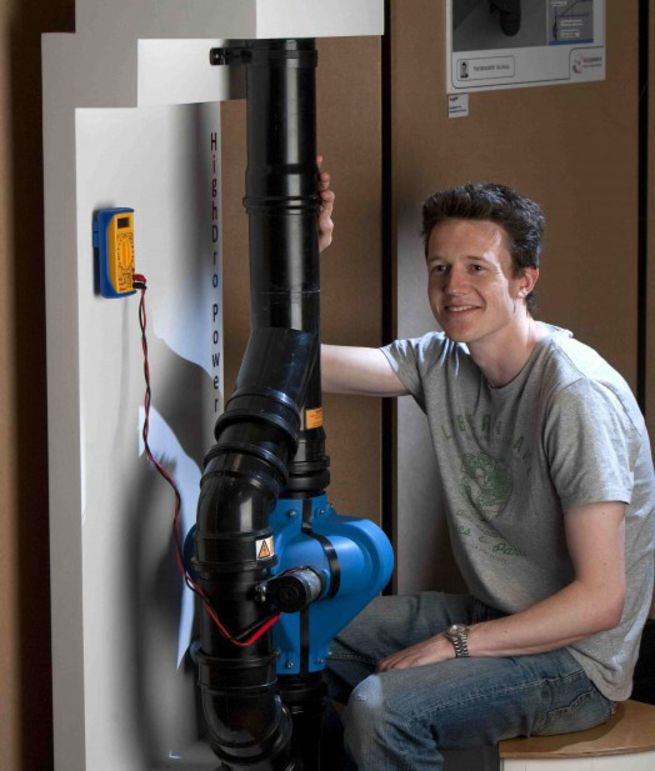
\includegraphics[width=7cm]{highDro.jpg}
\end{center}
Die Trinkwasserversorgung der obersten Stockwerke eines Hochhauses erfordert viel Druck (6-8 Bar). Da dieser Druck für die unteren Stockwerke zu gross ist, werden da Druckreduzierventile eingesetzt. Dabei bleibt viel Energie ungenutzt. Für diese Anwendung existieren schon Lösungen (z.Bsp. Arup LINK). Aber:
"Small-scale systems cannot easily generate enough power to justify their cost to large developers. The price per kilowatt-hour of generating power can be five times as high as simply buying it from the grid."(NEWYORKTIMES LINK)
\subsubsection{Fazit}
\clearpage 

\subsection{Energie}

\subsubsection{Recherchegrund}

Mit der Recherche über die Energie können wir abschätzen wie viel Energie gewonnen werden kann und welche Turbine dafür geeignet ist.

\subsubsection{Ergebnisse}

\paragraph{Berechnung}

Um Energie aus fliessendem Wasser zu gewinnen gibt es drei unterschiedliche Möglichkeiten/Turbinen: das Wasserrad, die Gleichdruckturbine und die Überdruckturbine. Wir haben uns entschieden, dass eine Gleichdruckturbine (Pelton-Turbine) für unsere Anwendung am besten geeignet ist.

\begin{center}
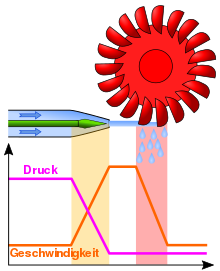
\includegraphics[width=5cm]{Gleichdruckturbine.png}
\end{center}

Das Wasser wird von einer gewissen Höhe in eine Fallleitung nach unten befördert. Die potenzielle Energie des Wassers wird dabei in kinetische Energie umgewandelt und das Wasser trifft mit einer Geschwindigkeit unten aus. Um diese Energie zu nutzen wird der Wasserstrahl auf die Schaufeln der Pelton-Turbine gerichtet, die anschliessend zu drehen beginnt.
\newline
\newline 
\newline
Die Endgeschwindigkeit des Wassers kann mit folgender Formel berechnet werden:
\begin{center}
\(v = \sqrt{2 \cdot g \cdot h} \)
\end{center}

Die Einheit der Geschwindigkeit \(v\) ist \si{m/s}. Das Schwerefeld \(g\) auf der Erde besitzt den Wert 9.81~\si{N/Kg}. Und die Höhe \(h\) hat die Einheit \si{m}.
\newline 
\newline 
\newline
Die Energie die gewonnen werden kann wird mit folgender Formel berrechnet:

\begin{center}
\(E =\frac 12\ \cdot m \cdot v^2\)
\end{center}

Die Energie  \(E\)  hat die Einheit  \si{J}. Die Einheit der Geschwindigkeit \(v\) ist \si{m/s} und die Masse \(m\) hat die Einheit \si{Kg}

\newpage

Um die Leistung zu erhalten, muss die Masse pro Zeit(1s) einberechnet werden. Die Masse wird  mit der Dichte und dem Volumenstrom ersetzt.

\begin{center}
\(P =\frac 12\ \cdot \varphi \cdot Q \cdot v^2\)
\end{center}

Die Leistung \(P\) hat die Einheit \si{W}. Der Volumentstrom \(Q\) hat die Einheit \si{m^3/s}. Die Einheit der Dichte \(\varphi\) ist \si{Kg/m^3} und die Einheit der Geschwindigkeit \(v\) ist \si{m/s}.
\newline 
\newline
 \newline


Mit diesen physikalischen Grundlagen kann nun die Leistung in Abhängigkeit der Höhe und des Volumenstromes berechnet werden. 

\begin{center}
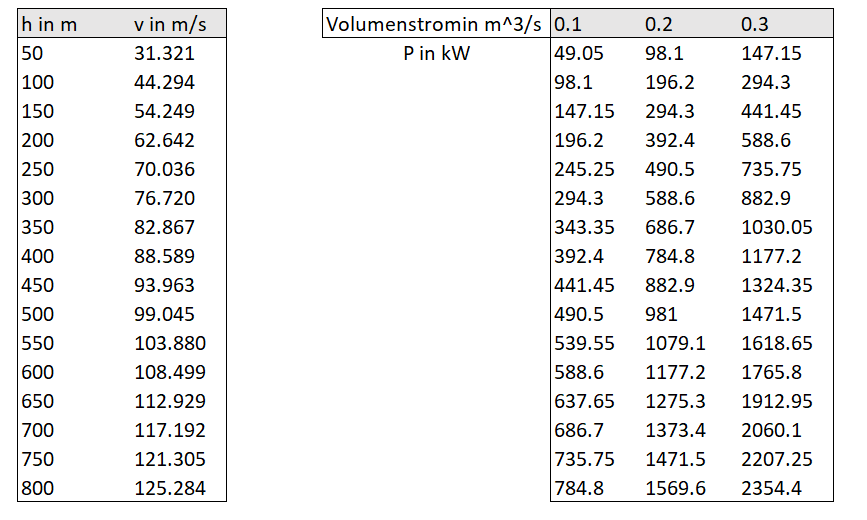
\includegraphics[width=10cm]{Leistungsberechnung.png}
\end{center}

Dies ist nur die Theoretische Leistung. Mit der Reibung am Rohr und dem Widerstand der Luftsäule wird das Wasser stark abgebrämst. Gemäss dem IZEG, die Versuche mit der Fallgeschwindigkeit durchgeführt haben, wird das Wasser bereichts nach 15m nicht mehr mehrklich schneller.

\begin{center}
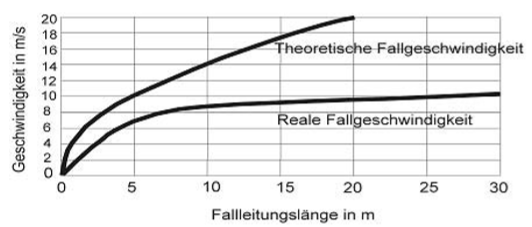
\includegraphics[width=10cm]{Fallgeschwindigkeit.png}
\end{center}

Mit der Endgeschwindigkeit von 10 \si{m/s}. wird bei einem Volumenstrom von 0.1 \si{m^3/s} noch 5 \si{kW} erzeugt.

\subsubsection{Fazit}

Die gewonnene Leistung nimmt ab ca. 15m nicht mehr merklich zu. Der Grundgedanke, dass die Geschwindigkeit des Wassers in grossen Fallhöhen zunimmt, funktioniert nur, wenn die Fallleitung komplett mit Wasser befüllt wäre und somit der Luftwiderstand wegfällt.

Damit man mit diesem System trotzem Energie zurückgewinnen kann, müsste all 15m eine Turbine die Energie des Wassers umwandeln.

\clearpage 






%\subsection{Turbine}

TODO: Pascal

\subsubsection{Recherchegrund}


\subsubsection{Ergebnisse}



\subsubsection{Fazit}

\clearpage 






\subsection{Infrastrukturen}

\subsubsection{Recherchegrund}

Mit der Recherche über bestehende Infrastrukturen in Hochhäusern können wir beurteilen, wie unsere Turbine am besten darin integriert wird.



\subsubsection{Ergebnisse}

\paragraph{Fachbegriffe}



\begin{table}[h]

\begin{tabular}{|l|l|lll}

\cline{1-2}

Fallleitung   & \begin{tabular}[c]{@{}l@{}}Eine senkrecht nach unten führende Abwasserleitung, führt meist in\\   Grundleitung oder Sammelleitung\end{tabular}                                                                                                      &  &  &  \\ \cline{1-2}

Verziehung    & Seitliche Versetzung einer Fallleitung                                                                                                                                                                                                              &  &  &  \\ \cline{1-2}

Sammelleitung & \begin{tabular}[c]{@{}l@{}}Horizontale Abwasserleitung, die innerhalb eines Gebäudes mehrere\\   Abwasserquellen zusammenführt\end{tabular}                                                                                                         &  &  &  \\ \cline{1-2}

Grundleitung  & \begin{tabular}[c]{@{}l@{}}Horizontale Abwasserleitung, die unter dem Gebäude oder auf dem\\   Grundstück im Boden verlegt sind; Unterste Leitung auf Privatgrundstück. \\ (https://www.haustechnikdialog.de/SHKwissen/1835/Grundleitung)\end{tabular} &  &  &  \\ \cline{1-2}

Hochhaus      & \begin{tabular}[c]{@{}l@{}}Schweiz: Gebäude mit einer Gesamthöhe von über 30 Metern.\\   Deutschland: Gebäude mit\\   einem Aufenthaltsraum, dessen Fussboden mindestens 22 Meter über dem Erdboden\\   liegt.\end{tabular}                         &  &  &  \\ \cline{1-2}

Nennweite     & Innendurchmesser eines Rohrs                                                                                                                                                                                                                        &  &  &  \\ \cline{1-2}

\end{tabular}

\end{table}



\paragraph{Fallleitungen, Beruhigungsstrecken und Verziehungen}

Durch Luftwiderstand und Reibung im Rohr beträgt die maximale Fallgeschwindigkeit, die in einer Fallleitung erreicht wird etwa 10 m/s und wird nach einer Fallhöhe von etwa 15 Metern erreicht. Daher muss auch in Hochhäusern das Abwasser erst am Ende einer Fallleitung abgebremst werden, unmittelbar bevor es einer Sammel- oder Grundleitung zugeführt wird. Die Abbremsung erfolgt durch eine sogenannte Beruhigungsstrecke, zwei 45° Winkel mit einem Zwischenstück von 250 mm am Ende der Fallleitung. Unsere Turbine sollte deshalb vor oder anstelle dieser Beruhigungsstrecke eingebaut werden.

(https://www.baunetzwissen.de/gebaeudetechnik/fachwissen/entwaesserung/abwasserleitungen-verlegung-2459057)



\begin{center}

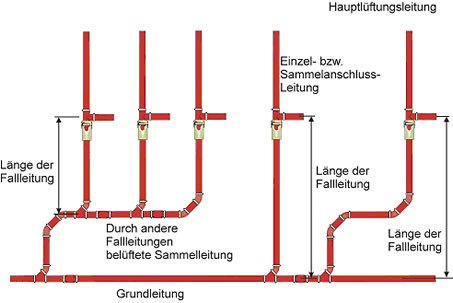
\includegraphics[width=10cm]{Falleitungen_1.jpg}

\end{center}

(https://www.baunetzwissen.de/imgs/1/3/0/5/2/1/7/487b6d4a778e66d0.jpg)



Da durch bauliche Gegebenheiten nicht immer ein Senkrechter Verlauf der Fallleitung möglich ist, sind Verziehungen erforderlich. Eine Verziehung ist eine Horizontale Versetzung der Fallleitung. ( https://docplayer.org/71335169-Schmutzwasser-fallleitungen-in-hochhaeusern.html, Seite 9)

Bei einer Verziehung kommt es auch zur Abbremsung des fallenden Abwassers. Deshalb sollte in den Letzten 15 Metern über der Turbine keine Verziehung mehr vorhanden sein, damit das Abwasser seine maximale Fallgeschwindigkeit erreichen kann.



\paragraph{Entlüftung}

In Fallleitungen werden grosse Luftvolumen bewegt, bei einer Nennweite DN 100 und einer Abwasserbelastung von beispielsweise 100 l/min werden 2340 l/min Luft mitgeführt.





(https://docplayer.org/71335169-Schmutzwasser-fallleitungen-in-hochhaeusern.html, Seite 3)

Diese Luftmenge behindert den Fluss des Abwassers, weshalb die Rohrleitungen belüftet werden müssen, damit ein Luftaustausch stattfinden kann. Auch muss verhindert werden, dass in den Leitungen Über- oder Unterdruck entsteht, da sonst ein Siphon leer gesaugt werden könnte. Dazu gibt es mehrere Lösungen, wobei nicht alle dazu geeignet sind, unsere Turbine einzubauen. Ein Geberit Sovent Formstück braucht wenig Platz, keine zusätzlichen Entlüftungsrohre und erlaubt mehr Durchfluss, da der Druckausgleich innerhalb Fallleitung geschieht. Es wird in jedem Stockwerk eingebaut und führt die Sammelleitungen des Stockwerkes in die Falleitung ein. Dies hat aber für uns aber den Nachteil, dass das Abwasser in jedem Stockwerk abgebremst wird und so nie seine Maximalgeschwindigkeit erreicht.

\begin{center}

\includegraphics[width=5cm]{Geberit_PE_Sovent_Formstück.jpg}

\end{center}

(https://www.geberit.ch/produkte/rohrleitungssysteme-entwaesserung/geberit-pe-abwasserrohre/)

Die anderen üblichen Entlüftungsarten sollten für uns kein Problem darstellen, da das Wasser im Fall nicht gebremst wird.


Direkte Nebenlüftung:

\begin{center}

\includegraphics[width=5cm]{Direkte_Nebenlüftung.PNG}

\end{center}

Indirekte Nebenlüftung:

\begin{center}

\includegraphics[width=5cm]{Indirekte_Nebenlüftung.PNG}

\end{center}

Sekundärlüftung:

\begin{center}

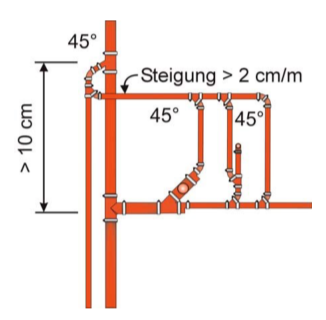
\includegraphics[width=5cm]{Sekundärlüftung.PNG}

\end{center}

(https://docplayer.org/71335169-Schmutzwasser-fallleitungen-in-hochhaeusern.html)





\subsubsection{Fazit}



\clearpage 







\subsection{Integrationen Bestehende Systeme}

\subsubsection{Recherchegrund}


\subsubsection{Ergebnisse}

Der in einer Photovoltaikanlage erzeugte Strom wird zunächst für den Eigenverbrauch genutzt. Das heißt, aktive Stromverbraucher, wie beispielsweise Kühltruhen oder andere Haushaltsgeräte, werden mit dem Strom betrieben. Steht jedoch mehr Strom als gebraucht zur Verfügung, fließt der überschüssige Solarstrom in die Batterie des Speichers - und dieser wird geladen. Erst wenn der Solarspeicher voll ist, wird der nicht benötigte Solarstrom ins Stromnetz eingespeist.
Wird in den Abend- oder Nachtstunden dann Strom benötigt, steht der gespeicherte Solarstrom zur Verfügung. Ist der Strombedarf tagsüber höher als die von der Photovoltaikanlage produzierte Menge Solarstrom, steht ebenfalls der gespeicherte Strom zur Verfügung - egal ob der Speicher vollständig oder nur teilgeladen ist. Erst wenn der gespeicherte Solarstrom ebenfalls nicht ausreicht, wird weiterer Strom vom Energieversorger bezogen.
Ein Großteil der am Markt erhältlichen Stromspeicher lässt sich nicht ohne weiteres in Bestandsanlagen integrieren. Meist sind technische Veränderungen, wie der Austausch des Wechselrichters oder Zusatzarbeiten notwendig. Ein hohes Gewicht und teilweise enorme Abmessungen vieler Energiespeicher für Strom schränken die Abstellmöglichkeiten ein und bringen einen großen Installationsaufwand mit sich: In der Regel sind mehrere Installateure mindestens einen Tag beschäftigt.

Wechselrichter
In einigen europäischen Ländern wird auf der Netzseite eine so genannte Einrichtung zur Netzüberwachung mit zugeordneten Schaltorganen (ENS) benötigt, die den Wechselrichter bei einer ungewollten Inselbildung abschaltet. Bei Anlagen mit installierten Leistungen über 30 \si{kW} kann auf die ENS verzichtet werden. Dort genügt eine Frequenz- und Spannungsüberwachung mit allpoliger Abschaltung zur sicheren Trennung vom Netz, falls dieses abgeschaltet wird bzw. ausfällt. 
Es wird oft mit einem hohen Wirkungsgrad der Wechselrichter geworben. Im Teillastbereich ist er etwas geringer und wird deshalb gemittelt und dann als „Europäischer Wirkungsgrad“ bezeichnet. Der Wirkungsgrad des Wechselrichters entscheidet jedoch nicht allein über den Gesamtwirkungsgrad einer Photovoltaikanlage. 
Seit Januar 2009 müssen Photovoltaikanlagen in Deutschland mit installierten Leistungen ab 100 \si{kW} über die Möglichkeit verfügen, vom Netzbetreiber in der eingespeisten Wirkleistung reduziert zu werden (§ 6.1 EEG). Des Weiteren besteht die Möglichkeit, dass eine bestimmte Menge Blindleistung zur Verfügung gestellt wird. In der Praxis werden diese Vorgaben dynamisch über Rundsteuerempfänger realisiert, die eine vierstufige Wirkleistungsreduzierung signalisieren können bzw. einen von 1 abweichenden Wirkfaktor von beispielsweise $\cos \phi = 0,95$ (induktiv) vorgeben. Durch die Bereitstellung von induktiver Blindleistung können kapazitiv bedingte Überspannungen vermieden werden.[3] 
Ab Juli 2011 müssen auch kleinere Anlagen im Niederspannungsnetz vergleichbare Regelfunktionen anbieten.[4] Landestypische weitergehende Vorschriften führen zu Lieferengpässen und höheren Erzeugungskosten. Gegenkonzepte wie Net Metering verfolgen einen unkomplizierteren Ansatz und verlagern die Problematik auf den Netzbetreiber. 
Bei größeren Anlagen, bei welchen unter anderem die Mittelspannungsrichtlinie einzuhalten ist, sind weitere Maßnahmen zu dynamischen Netzstabilisierung wie die Fähigkeit zu Low-Voltage Ride Through vorgeschrieben. Die Maßnahmen dienen dazu um eine ungewollte und gleichzeitige Abschaltung vieler Anlagen bei kurzzeitiger lokaler Unterspannung, wie sie im Rahmen von Kürzschlüssen oder anderen Fehlern im Drehstromsystemen vorkommen, zu vermeiden. 
Einphasige Anlagen dürfen in Deutschland nur bis zu einer maximalen Leistung von 5 \si{kW} (4,6 \si{kW} Dauerleistung) in das Stromnetz einspeisen.[5] Diese Beschränkung dient der Netzstabilität und vermeidet Schieflasten. Neben der grundlegenden Funktion der Energiewandlung verfügt ein Solarwechselrichter über eine umfangreiche Datenerfassung und zum Teil Möglichkeiten zur Fernwartung. 



\subsubsection{Fazit}
Stromspeicher sind teuer – nicht nur wegen der Batteriezellen, sondern auch wegen zugehöriger Hardware. Es ist fraglich, ob es diese Investition angesichts der überschaubaren Energiemenge wert ist. 
Die Einspeisung des Stromes in das Stromnetz scheint hingegen schon eher möglich zu sein, da dies in der Schweiz ohne Bewilligung erlaubt ist, solange die eingespiesene Leistung gering ist. Dazu muss der Strom zunächst gleichgerichtet und anschliessend von einem Wechselrichter auf 230\si{V} @ 50 \si{Hz} transformiert werden. Solche Gerät sind erhältlich, bewegen sich preislich aber zwischen mehreren hundert bis mehreren tausend Franken.
Die Integration in bestehende Solaranlagen ist vermutlich die einfachste Option, da in diesem Fall Energiespeicher und/oder Wechselrichter meist schon vorhanden sind.


\clearpage 






\subsection{Sicherheit}


\subsubsection{Recherchegrund}
Wir möchten über die Sicherheit der Abwasserrohre und die entstehenden Abgase recherchieren, um gewisse Risiken einschätzen zu können. 
\subsubsection{Ergebnisse}
Die Verstopfungsgefahr in den Abwasserrohren ist sehr klein. %es geht ja nicht nur um die Verstopfung in Rohren ohne Turbine. Es geht besonders um die Verstopfung mit Turbine. Dies scheint ein verbreitetes Problem zu sein. Vielleicht kannst du verschiedene Verstopfungsarten/Gefahren für Turbinen auflisten. Zsbp Haare oder tampons usw. Auch die Abnutzung durch Kalk usw müsste studiert werden.
Eine Verstopung passiert selten, weil das Schmutzwasser nur geringen Abständen in das Rohr hineinfliesst. Die Möglichkeit besteht, diese Verstopfungen ganz zu eliminieren, in dem man eine Hebeanlage in den Toilettenräumen einbaut. Mit diesen Hebeanlagen entsteht aber zusätzlicher Lärm. In diesen Bereichen werden flexible Rohre benützt, um Rohrbrüche zu vermeiden.
\paragraph{Leitungen}
Bei Fallleitungen die Grösser als 10 bis 20\si{m} sind, schreibt die Norm, dass man zwei 45°-Bögen mit einem geraden Stück von 250\si{mm} Länge zum Druckabbau eingebaut werden. Heutzutage kann man die Rohre so wählen, dass gar kein Rohrbruch entsteht.
\paragraph{Abgase}
Die Abgase (Schwefelgas) die entstehen, werden Mittels zusätzlicher Lüftungsleitung abgeleitet und über das Dach in die Umwelt gelassen. In den Hebeanlagen kann es durch Gärprozesse zur Gasbildung kommen. Den dadurch entstehenden Unterdruck im Raum muss man durch Lüftung selber regeln. 
\paragraph{Berechnung}
Wartungstechnisch werden Abwasserrohre alle fünfzehn Jahre auf Dichtigkeit kontrolliert. Die Rohre werden so gewählt, dass sie ein Leben lang halten.

\subsubsection{Fazit}

Die Sicherheit ist in vielen Bereichen gewährleistet. Wenn die Fallleitung einen 45° Bogen hat, wirkt sich das auf die Fliessgeschwindigkeit des Schmutzwassers und somit negativ auf die Energiegewinnung aus. Zusätzlich wird mit der Installation einer Hebeanlage Energie aus dem Netz bezogen und Lärm verursacht.%Ist also nicht gerade sehr positiv. Gibt es andere Arten Verstopfungen zu vermeiden? Zbsp optimierte Beschaufelung der Turbine? 

\clearpage 











\section{Zusammenfassung}



\section{Quellenverzeichnis}



\section{Echtheitserklärung}





%%---NOTES for DEBUG---------------------------------------------------------------------
\ifdraft{%Do this only if mode=draft
%%requires \usepackage{todonotes})
\newpage
\listoftodos[\section{Todo-Notes}]
\clearpage
}
{%Do this only if mode=final
}
\end{document}
